\chapter{UI Overview}
\label{sec:ui_overview}

In this section, the main GUI components are described, to give an overview and introduce the different workflow options.

\subfile{ui_main_window}

\section{Main Menu}
\label{sec:main_menu}

\subsection{File Menu}
\label{sec:ui_overview_file_menu}

Databases can be created, opened and closed using the 'File' menu.

\begin{figure}[H]
    \includegraphics[width=6cm,frame]{figures/ui_file_menu.png}
  \caption{File Menu}
\end{figure}

\begin{itemize}
 \item New: Create new database file
 \item Open: Open existing database file
 \item Open Recent: Open recent existing database file
 \item Export: Export the currently opened database into a new database file
 \item Close: Close current database
 \item Save Config: Save current configuration
 \item Quit Without Saving Config: Quit application without saving configuration
 \item Quit: Quit application and save configuration
\end{itemize}
\  \\

After a database was created or opened, the 'Context' and 'Import' menus become available.

\subsection{Context Menu}
\label{sec:ui_overview_context_menu}

The Context menu manages the active Data Context. It sits between the 'File' and 'Import' menus. The menu title in the menu bar is the name of the active Data Context, or 'No Context' when none is active.

\begin{figure}[H]
    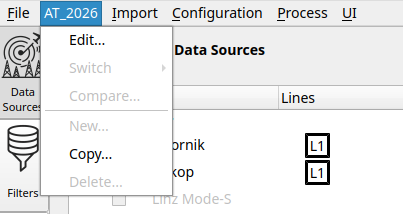
\includegraphics[width=8cm,frame]{figures/ui_context_menu.png}
  \caption{Context Menu}
\end{figure}

\begin{itemize}
 \item Edit...: Opens the Data Context dialog
  \begin{itemize}
   \item see \nameref{sec:configure_data_context}
  \end{itemize}
 \item Switch: Submenu listing all other available contexts; selecting one activates it. Disabled when no other contexts exist.
 \item Compare...: Compare contexts. Currently disabled.
 \item New...: Creates a new empty context and activates it
 \item Copy...: Copies a context under a new name
 \item Delete...: Deletes one or more contexts. Disabled when only one context remains.
\end{itemize}
\  \\

Please \textbf{note} that when no Data Context is available (e.g. after deleting the last one), the application runs in the 'No Context' state with reduced menu availability until a new context is created or imported. \\

\subsection{Import Menu}
\label{sec:ui_overview_import_menu}

Data can be imported into the database using the 'Import' menu. This menu is only accessible if a database has been opened.

\begin{figure}[H]
  \center
    \includegraphics[width=8cm,frame]{figures/ui_import_menu.png}
  \caption{Import Menu}
\end{figure}

\begin{itemize}
 \item ASTERIX Recording: Import ASTERIX recording file
 \begin{itemize}
 \item see \nameref{sec:ui_import_asterix}
 \end{itemize}
 \item PCAP Network Recording: Import ASTERIX from a PCAP network recording
  \begin{itemize}
 \item see \nameref{sec:ui_import_pcap}
 \end{itemize}
 \item ASTERIX From Network: Import ASTERIX from network interfaces in Live mode
  \begin{itemize}
 \item see \nameref{sec:ui_import_asterix_network}
 \end{itemize}
 \item JSON Recording: Import JSON recording file
  \begin{itemize}
 \item see \nameref{sec:ui_import_json}
 \end{itemize}
 \item GPS Trail: Import (D)GPS trail from NMEA file
  \begin{itemize}
 \item see \nameref{sec:ui_import_gps}
 \end{itemize}
 \item View Points: Import View Points definition file
  \begin{itemize}
 \item see \nameref{sec:ui_import_viewpoints}
 \end{itemize}
\end{itemize}
\  \\

\subsection{Configuration Menu}
\label{sec:ui_overview_config_menu}

The 'Configuration' menu exposes program-wide options. The active Data Context (data sources, sector layers, FFTs, ASTERIX configuration and colors) is managed through the 'Context' menu, see \nameref{sec:ui_overview_context_menu}.

\begin{figure}[H]
    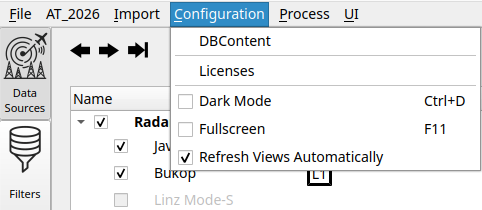
\includegraphics[width=8cm,frame]{figures/ui_configuration_menu.png}
  \caption{Configuration Menu}
\end{figure}

\begin{itemize}
 \item DBContent: Display all Meta Variables and DBContent variables
  \begin{itemize}
   \item see \nameref{sec:configure_show_content}
  \end{itemize}
 \item \nameref{sec:ui_configure_licenses}: Manage licenses
 \item \nameref{sec:ui_overview_dark_mode}: Enable/Disable dark mode
 \item Fullscreen: Toggles full-screen display of the main window
 \item Refresh Views Automatically: Sets if views should trigger an automatic data reload process when any configuration changes are made (e.g. adding a DBContent variable in Table View)
\end{itemize}
\  \\

\subsection{Process Menu}
\label{sec:ui_overview_process_menu}

Post-processing tasks can be performed using the 'Process' menu. This menu is only accessible if a database was opened.

\begin{figure}[H]
  \center
    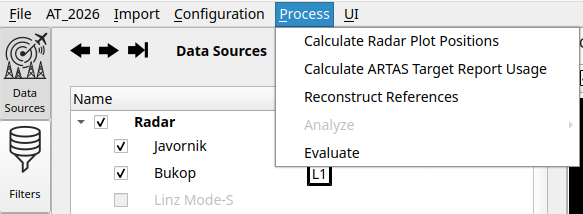
\includegraphics[width=10cm,frame]{figures/ui_process_menu.png}
  \caption{Process Menu}
\end{figure}

\begin{itemize}
 \item \nameref{sec:ui_proc_radar_plot_pos}: (Re-)Calculate Radar plot position information
 \item \nameref{sec:ui_associate_tr_artas}: Associate used target reports to ARTAS tracks based on ARTAS TRI information
 \item \nameref{sec:ui_proc_reconst_references}: Find unique targets, associate target reports and calculate reference trajectories
 \item Analyze: Submenu providing per-DSType data-source analysis tasks
  \begin{itemize}
   \item MLAT: Analyze one or more MLAT data sources (data items, sensor coverage / PD, position accuracy); see \nameref{chap:analyze}
  \end{itemize}
 \item \nameref{sec:ui_proc_evaluate}: Run a new Evaluation
\end{itemize}
\  \\

Please \textbf{note} that further DSType-specific analysis entries will be added in future releases. \\

\subsection{UI Menu}
\label{sec:ui_overview_ui_menu}

The UI can be reset to a "default" state (as it existed at application startup) using the 'Reset Views' function.

\subfile{import/ui_import}
\subfile{config/ui_configuration}
\subfile{process/ui_process}
\subfile{ui_ui}
\subfile{ui_views}

\section{Dark Mode}
\label{sec:ui_overview_dark_mode}

After Dark Mode is enabled or disabled, the GUI switches to a dark theme. The toggle takes effect immediately, no application restart is required. Dark Mode can be enabled either via the 'Configuration' menu entry or with the 'Ctrl+D' keyboard shortcut.

\begin{figure}[H]
  \hspace*{-2.5cm}
    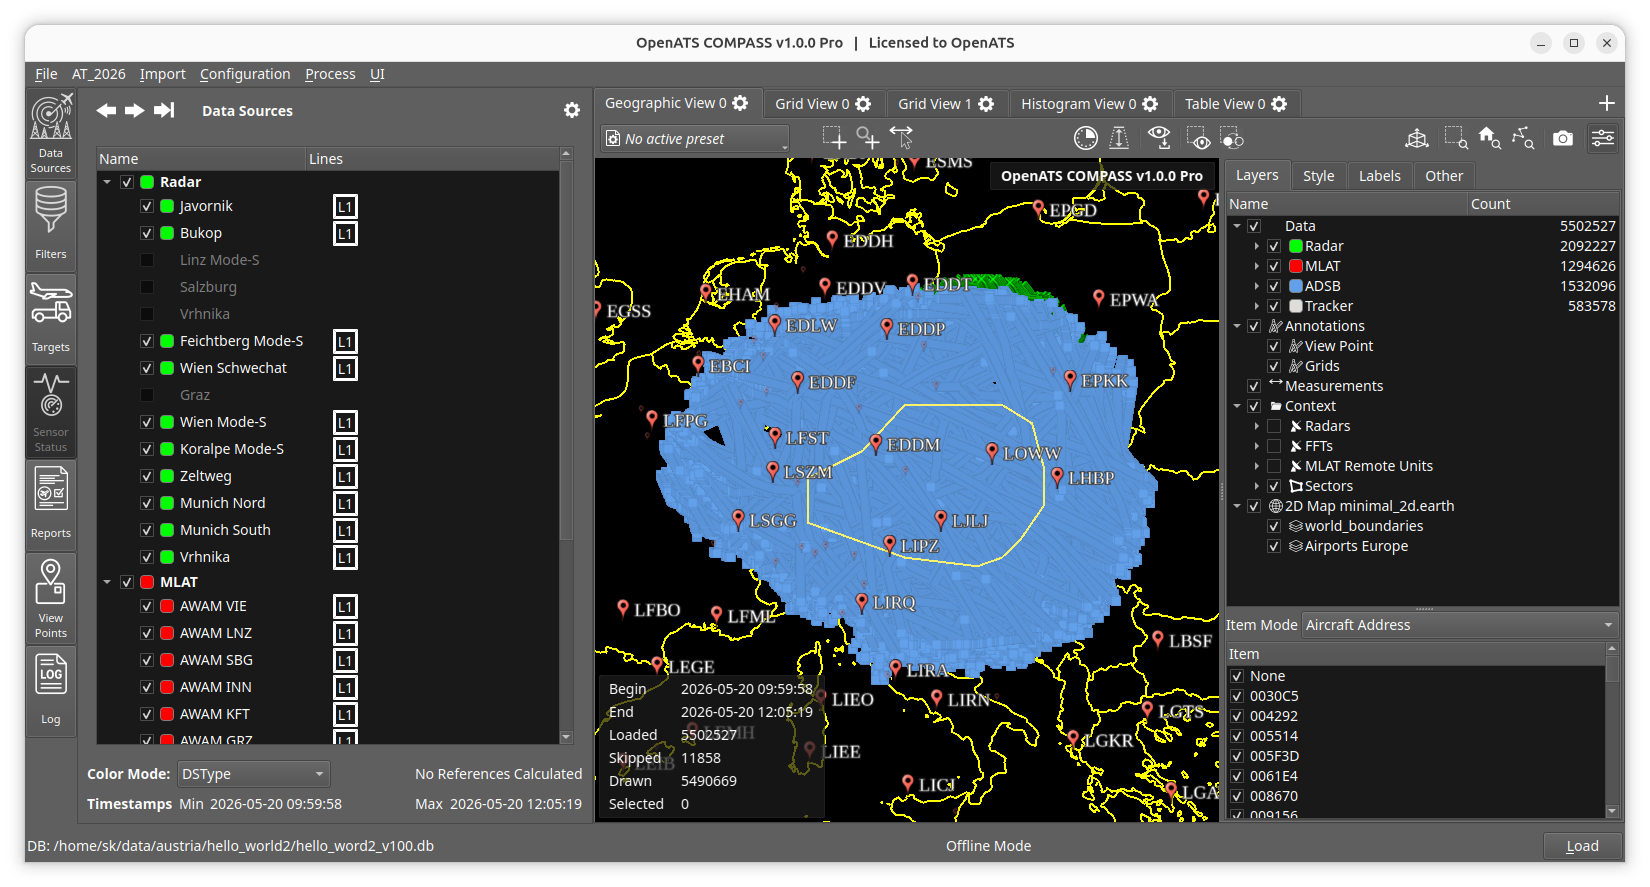
\includegraphics[width=19cm]{figures/dark_mode.png}
  \caption{Main Window Dark Mode}
\end{figure}

Readability of GUI elements in Dark Mode has been improved compared to earlier releases. Please \textbf{note} that some Views may still show minor coloring inconsistencies in special cases. Please also \textbf{note} that the window decoration color can only be changed using your Linux window manager settings. \\

There also exist special dark mode maps for Geographic View as described in \nameref{ref:geoview_map_osm_dark}.

